\chapter{Analysis}
	[TODO:felvezets]
	\section{Self driving car variations}
		To test the effect of autonomous drivers in traffic, the same red traffic light situation was implemented. However in this case one of the driver's parameters have been substituted with an autonomous driver parameters. The most representative figure of the result of this task is where the count of cars passed the target line - 100 meters - is illustrated as a function of time. Cars one by one have been exchanged and then simulated with the reaming cars. So a total of ten simulations were run. The result can be seen on Figure \ref{fig:vehicle_density}.
		\begin{figure}[ht]
			\centering
			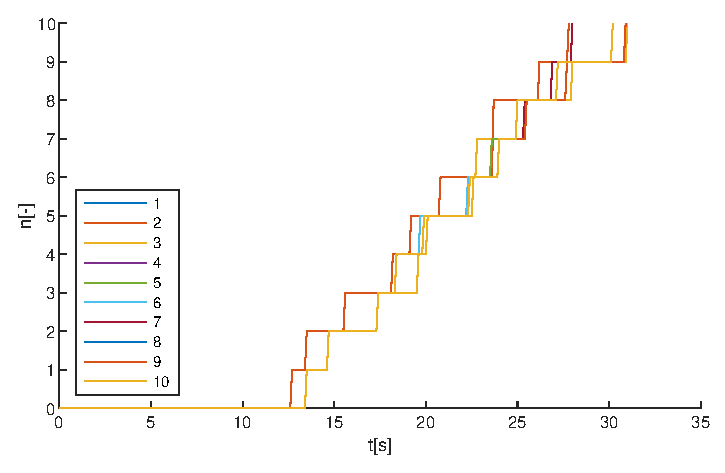
\includegraphics[width=0.75\textwidth]{eemobil/vehicle_density}
			\caption{Vehicles passes the target line}
			\label{fig:vehicle_density}
		\end{figure}

		As Figure \ref{fig:vehicle_density} shows the first car reaches the target line in ~13 seconds. The interesting part is at the top right corner of the figure, where it can be seen that depending on which car has been exchanged the overall elapsed time can change up to 10 \%. The minimum, maximum, average and standard deviation values can be found in Table \ref{tab:vehicle_density_minmaxavg_case1}.
		In the hope of a better figure the same simulation results are shown on Figure \ref{fig:vehicle_density_avg} with averaged representation. It is slightly better than previously.
		\begin{table}[ht]
			\begin{center}
				\begin{tabular}{ |c|c|c|c|}
					\hline
					\vehicledensitytable{1}
					\hline
				\end{tabular}
			\end{center}
			\caption{Time until the last car has reached the target line. 1 autonomous car}
			\label{tab:vehicle_density_minmaxavg_case1}
		\end{table}
		\begin{figure}[ht]
			\centering
			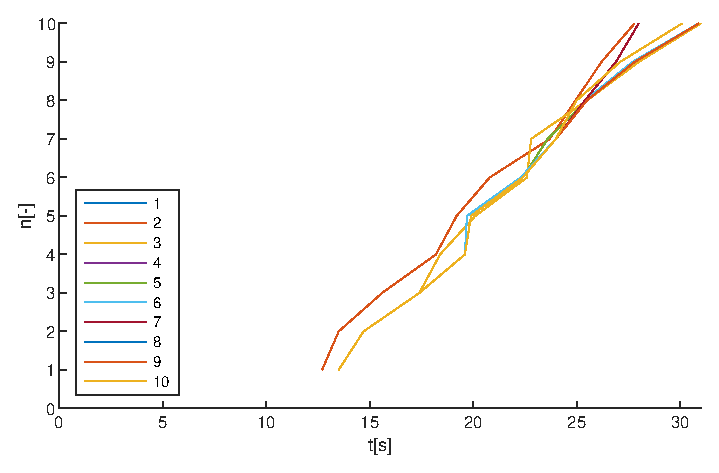
\includegraphics[width=0.75\textwidth]{eemobil/vehicle_density_avg}
			\caption{Vehicles passes the target line}
			\label{fig:vehicle_density_avg}
		\end{figure}
		
		The previous simulations were run with only one self-driving car but in different positions. It can be seen that one autonomous driver could make the traffic faster. Based on the position of that one car it will mostly decrease the overall duration. 
		
		Let us try the same simulation but this time run it exchange two drivers to autonomous driver see how will improve the situation. The total number of 45 unique combinations were simulated.
		\begin{table}[ht]
			\begin{center}
				\begin{tabular}{ |c|c|c|c|}
					\hline
					\vehicledensitytable{2}
					\hline
				\end{tabular}
			\end{center}
			\caption{Time until the last car has reached the target line. Two autonomous car}
			\label{tab:vehicle_density_minmaxavg_case2}
		\end{table}
		
		The same simulations were run with three self-driving cars as well. The total number of 120 unique combinations were simulated.
		\begin{figure}[ht]
			\centering
			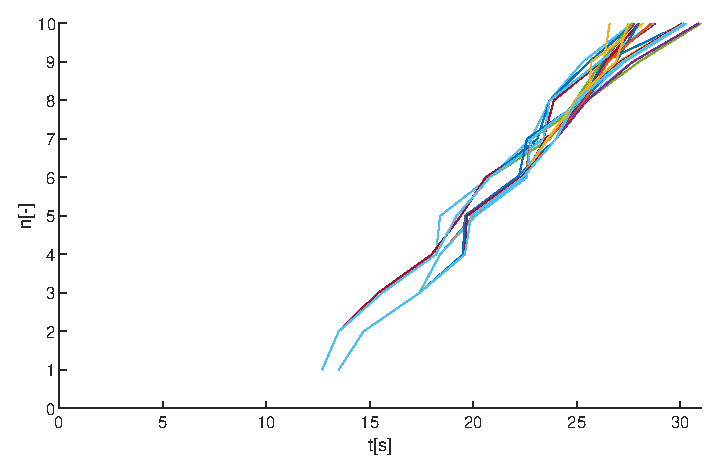
\includegraphics[width=0.75\textwidth]{eemobil/vehicle_density_case_2}
			\caption{Number of vehicles passes the target line with two self-driving cars}
			\label{fig:vehicle_density_case_2}
		\end{figure}
		\begin{table}[ht]
			\begin{center}
				\begin{tabular}{ |c|c|c|c|}
					\hline
					\vehicledensitytable{3}
					\hline
				\end{tabular}
			\end{center}
			\caption{Time until the last car has reached the target line. Three autonomous car}
			\label{tab:vehicle_density_minmaxavg_case3}
		\end{table}
		\begin{figure}[ht]
			\centering
			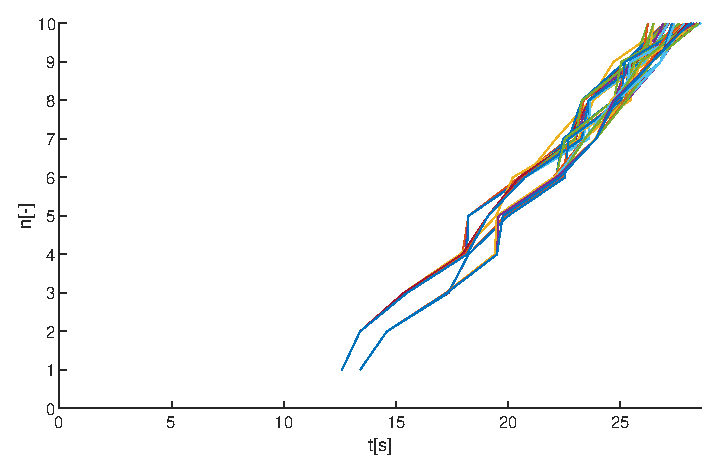
\includegraphics[width=0.75\textwidth]{eemobil/vehicle_density_case_3}
			\caption{Number of vehicles passes the target line with three self-driving cars}
			\label{fig:vehicle_density_case_3}
		\end{figure}
		
		\begin{figure}
			\centering
			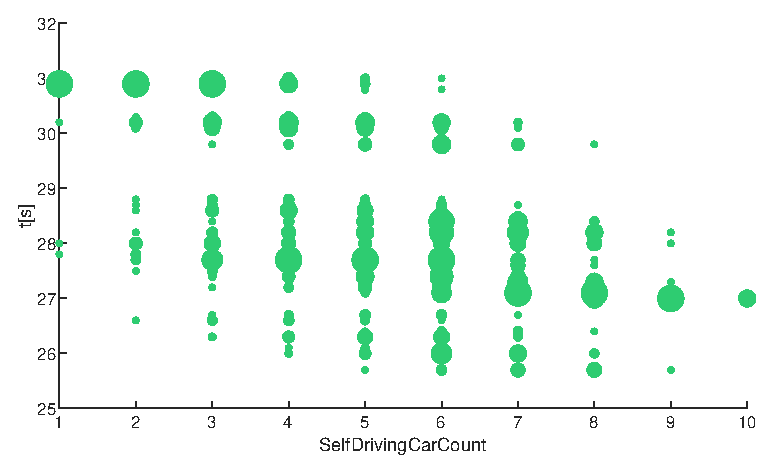
\includegraphics[width=0.8\textwidth]{eemobil/variations}
			\caption{Time variation of autonomous drivers}
			\label{fig:self_variations}
		\end{figure}
		\begin{figure}
			\centering
			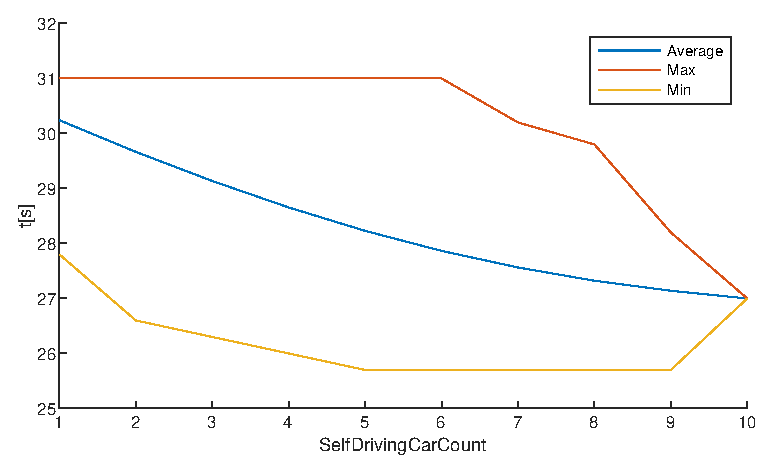
\includegraphics[width=0.8\textwidth]{eemobil/variations_avgminmax}
			\caption{Average, minimum and maximum of elapsed time.}
			\label{fig:self_variations_avgminmax}
		\end{figure}
		\begin{figure}
			\centering
			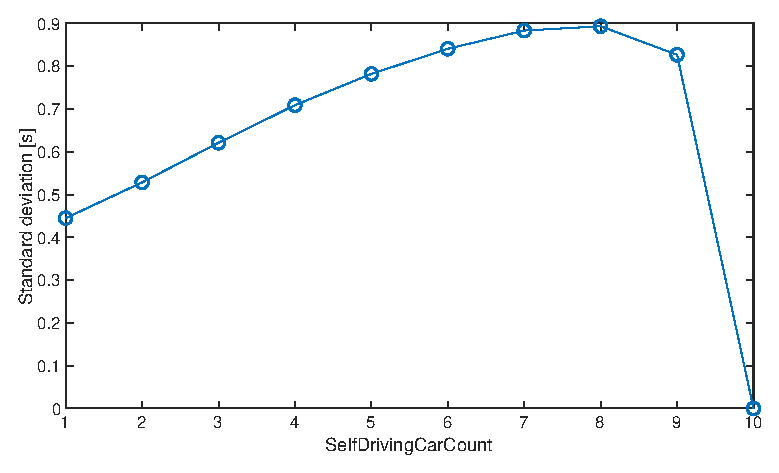
\includegraphics[width=0.8\textwidth]{eemobil/variations_std}
			\caption{Standard deviation of elapsed time}
			\label{fig:self_variations_std}
		\end{figure}
